 %+ !TeX encoding = UTF-8
% !TeX spellcheck = fr-FR
\documentclass[a4paper,french,final]{memoir}
\usepackage{luacode}
\usepackage[german,main=french]{babel}
\usepackage[autostyle=true,maxlevel=3]{csquotes}
\usepackage{microtype}
\usepackage{fontspec}
\usepackage{geometry}
\usepackage{mathtools} 
\usepackage[math-style=french,warnings-off={mathtools-colon,mathtools-overbracket}]{unicode-math}
\setmainfont{TeX Gyre Termes}
\setmathfont{TeX Gyre Termes Math}
\setmathfont[range=bb]{STIX Two Math}
\setmathfont[range={scr,cal}]{TeX Gyre Pagella Math}
\usepackage[amsmath,thmmarks,hyperref]{ntheorem}
\usepackage[most]{tcolorbox}
\usepackage{xparse,xpatch}
\usepackage{tikz}
\usepackage{caption}
\usetikzlibrary{calc,trees,positioning,arrows,fit,shapes,calc}
\usepackage{lualatex-math}
\usepackage[unicode,naturalnames]{hyperref}
\usepackage{cleveref}
\AtBeginDocument{\let\savedemptyset\emptyset} % 
\AtBeginDocument{\let\emptyset\varnothing} % 
\AtBeginDocument{\let\savedleq\leq} % 
\AtBeginDocument{\let\savedgeq\geq} %
\AtBeginDocument{\let\leq\leqslant} % 
\AtBeginDocument{\let\geq\geqslant} %
\newcommand{\paral}{\mathrel{\!/\mkern-5mu/\!}} % \parallel existe déjà : || vs //
\makeatletter
\newcommand*{\theauthor}{\@author}
\newcommand*{\thetitle}{\@title}
\newcommand*{\thedate}{\@date}
\renewcommand{\xmapsto}[2][]{\mathrel{\mathpalette\xmapsto@{{#1}{#2}}}}
\renewcommand{\xmapsto}[2][]{\mathrel{\mathpalette\xmapsto@{{#1}{#2}}}}
\newcommand{\xmapsto@}[2]{\xmapsto@@{#1}#2}
\newcommand{\xmapsto@@}[3]{%
  \begingroup
  \sbox\z@{$\m@th#1\mathop{}\limits_{\;#2\;}^{\;#3\;}$}%
  \mathop{\Uhextensible width \wd\z@ 0 "27FC}_{#2}^{#3}%
  \endgroup
}
\renewcommand{\xLeftrightarrow}[2][]{\mathrel{\mathpalette\xLeftrightarrow@{{#1}{#2}}}}
\newcommand{\xLeftrightarrow@}[2]{\xLeftrightarrow@@{#1}#2}
\newcommand{\xLeftrightarrow@@}[3]{%
  \begingroup
  \sbox\z@{$\m@th#1\mathop{}\limits_{\;#2\;}^{\;#3\;}$}%
  \mathop{\Uhextensible width \wd\z@ 0 "027FA}_{#2}^{#3}% 027FA code for long left right double arrow in unicode-math-table.tex 
  \endgroup
}

\newcounter{proofpart}
\newcommand{\proofpart}{\@ifstar{\@proofpart}{\@@proofpart}}

\newcommand{\@proofpart}[1]{%
  \if\detokenize{#1}\relax\else{
  \par
  \addvspace{\medskipamount}%
  \noindent \itshape%
  {#1~:\par\nobreak\smallskip}%
  \normalfont
  \@afterheading
}\fi
}

\newcommand{\@@proofpart}[1]{%
  \par
  \addvspace{\medskipamount}%
  \stepcounter{proofpart}%
  \noindent Partie \theproofpart~:~\itshape%
  \if\detokenize{#1}\relax%
  \else{#1.}\fi%
  \par\nobreak\smallskip
  \normalfont
  \@afterheading
}
\makeatother
%%%%%%%%%%%%%%%%%%%%%%%%%%%%%%%%%%%%%%%%%%%%%%%%
%            NUMEROTATION (CLASSE MEMOIR)       %
%%%%%%%%%%%%%%%%%%%%%%%%%%%%%%%%%%%%%%%%%%%%%%%%%
\setsecnumdepth{subsubsection}
\renewcommand{\cftpartaftersnum}{.}
\renewcommand{\cftchapteraftersnum}{.}
\renewcommand{\cftpartdotsep}{\cftdotsep}
\renewcommand{\cftchapterdotsep}{\cftdotsep}% Chapters should use dots in ToC
\aliaspagestyle{title}{empty} 
\aliaspagestyle{part}{empty} 
%\setlength\headheight{\dimexpr \headheight+0.20004pt}

\usepackage[backend=biber,style=alphabetic]{biblatex}
\addbibresource{references.bib}
%%%%%%%%%%%%%%%%%%%%%%%%%%%%%
%   THEOREMES SANS BOITES   %
%%%%%%%%%%%%%%%%%%%%%%%%%%%%%
\theoremstyle{break}
\theoremseparator{~:} % espace fine insécable avant le :
\newtheorem{lemma}{Lemme}
\newtheorem{corollary}{Corollaire}
\newtheorem{definition}{Définition}
\theoremstyle{plain}
\newtheorem*{question}{Question}
\newtheorem*{answer}{Réponse}
\newtheorem{remark}{Remarque}
\theoremsymbol{\text{\bsc{c.q.f.d}}} % mod
\theorembodyfont{\normalfont}
\theoremprework{\setcounter{proofpart}{0}}
\newtheorem*{proof}{Démonstration}
%%%%%%%%%%%%%%%%%%%%%%%%%%%%%
%            COULEURS       %
%%%%%%%%%%%%%%%%%%%%%%%%%%%%%
\definecolor{vert}{RGB}{0,181,0}
\definecolor{oran}{RGB}{223,74,0}
\definecolor{viol}{RGB}{134,0,175}
\definecolor{roug}{RGB}{215,15,0}
\definecolor{bleu}{RGB}{0,104,180}

%%%%%%%%%%%%%%%%%%%%%%%%%%%%%
%   BOITES POUR THEOREMES   %
%%%%%%%%%%%%%%%%%%%%%%%%%%%%%
\tcbset{separator sign={},
        description delimiters parenthesis,
        label separator=-,
styletheorem/.style={enhanced,
  coltitle=black,
  colback=white,
  fonttitle=\bfseries,
  boxrule=\fboxrule,
  boxed title style={boxrule=\fboxrule},
  attach boxed title to top left={yshift=-2mm, xshift=2mm},
    }%
}
\newtcbtheorem[auto counter, number within = section]
{theoremb}{Théorème}{styletheorem,colframe=roug,
colback=white!90!roug,colbacktitle=white!80!roug,label type=theorem}{thm}
\newtcbtheorem[auto counter, number within = section]
{remarkb}{Remarque}{styletheorem,colframe=oran,
colbacktitle=white!80!oran,colback=white!90!oran,label type=remark}{rem}
\newtcbtheorem[auto counter, number within = section]
{defb}{Définition}{styletheorem,colframe=bleu,
colbacktitle=white!80!bleu,colback=white!90!bleu,label type=definition}{def}
\newtcbtheorem[auto counter, number within = section]
{noteb}{Commentaire}{styletheorem,colframe=vert,
colbacktitle=white!80!vert,colback=white!90!vert,label type=note}{note}
% le label type fait automatiquement la jonction avec cleveref pour nommer les théorèmes : le dernier groupe (thm,rem,def) permet de créer des labels automatiquement. 

%%%%%%%%%%%%%%%%%%%%%%%%%%%%%%%%%%
%  SEPARATEUR (DANS LES PREUVES) : \proofpart   %
%%%%%%%%%%%%%%%%%%%%%%%%%%%%%%%%%%%
% une  commande est définie pour séparer les preuves en deux variantes : avec et sans étoiles. (\proofpart et \proofpart*)
% Par défaut, elle crée des sous parties dans un environement de démonstration sous la forme 
% " Partie n : [titre en italique]. ", où n est un entier naturel strictement positif. Dans le cas ou le titre est vide, le point (.) n'est pas ajouté. Si le titre est vide, il faut utiliser \proofpart{}
% Avec une étoile, on obtient 
%[titre en italique : ] 

\newcommand{\deffunct}[5]{%
\begin{align*}%
      #1 \colon & #2 \to #3\\
       &#4\xmapsto{\hphantom{#1}} #5
\end{align*}%
}
%%%%%%%%%%%%%%%%%%%%%%%%%%%%%
%   PAGE DE GARDE            %
%%%%%%%%%%%%%%%%%%%%%%%%%%%%%
\newcommand{\HRule}{\rule{\paperwidth}{0.5mm}} % trait, régler eppaisseur
\newcommand*{\theuniversity}{Université de Toulon}
\newcommand*{\theyearname}{Licence de Mathématiques, parcours mathématiques, 
2\ieme~année}
\newcommand*{\thesupervisor}{Joachim \bsc{Asch}}
\author{Anastasiia \bsc{Chernetcova}~\&~Tom \bsc{Domenge}}
\title{Projet TER 2020\par
            Dénombrabilité : \par $\mathbb{N},2\mathbb{N} \ \& \ \mathbb{Q}$\par}

%%%%%%%%%%%%%%%%%%%%%%%%%%%%%%%%%%%%%%%%%%%%%%
%   Opérateurs (dans le style de max etc.   %
%%%%%%%%%%%%%%%%%%%%%%%%%%%%%%%%%%%%%%%%%%%%%%
\DeclareMathOperator{\Card}{Card} % s'utilise avec \Card en mode maths
\makeatletter
\newcommand{\diagdenomb}{\@ifstar{\@diagdenomb}{\@@diagdenomb}}
\newcommand{\@diagdenomb}{\begin{figure}[htbp]
    \centering
\begin{tikzpicture}
\tikzstyle{keepstyle} =[rectangle, rounded corners, draw, fill=white]
\node at (0,0) {$\vdots$};
\node[keepstyle] (51) at (0,1) {$\frac{5}{1}$};
\node[keepstyle] (41) at (0,2) {$\frac{4}{1}$};
\node[keepstyle] (31) at (0,3) {$\frac{3}{1}$};
\node[keepstyle] (21) at (0,4) {$\frac{2}{1}$};
\node[keepstyle] (11) at (0,5) {$\frac{1}{1}$};
\node at (1,0) {$\vdots$};
\node[keepstyle] (52) at (1,1) {$\frac{5}{2}$};
\node at (1,2) {$\frac{4}{2}$};
\node[keepstyle] (32) at (1,3) {$\frac{3}{2}$};
\node at (1,4) {$\frac{2}{2}$};
\node[keepstyle] (12) at (1,5) {$\frac{1}{2}$};
\node at (2,0) {$\vdots$};
\node at (2,1) {$\frac{5}{3}$};
\node[keepstyle] (43) at (2,2) {$\frac{4}{3}$};
\node at (2,3) {$\frac{3}{3}$};
\node[keepstyle] (23) at (2,4) {$\frac{2}{3}$};
\node[keepstyle] (13) at (2,5) {$\frac{1}{3}$};
\node at (3,0) {$\vdots$};
\node at (3,1) {$\frac{5}{4}$};
\node at (3,2) {$\frac{4}{4}$};
\node[keepstyle] (34) at (3,3) {$\frac{3}{4}$};
\node at (3,4) {$\frac{2}{4}$};
\node[keepstyle] (14) at (3,5) {$\frac{1}{4}$};
\node at (4,0) {$\vdots$};
\node  at (4,1) {$\frac{5}{5}$};
\node at (4,2) {$\frac{4}{5}$};
\node at (4,3) {$\frac{3}{5}$};
\node[keepstyle] (25) at (4,4) {$\frac{2}{5}$};
\node[keepstyle] (15) at (4,5) {$\frac{1}{5}$};
\node at (5,0) {$\vdots$};
\node  at (5,1) {$\frac{5}{6}$};
\node at (5,2) {$\frac{4}{6}$};
\node at (5,3) {$\frac{3}{6}$};
\node at (5,4) {$\frac{2}{6}$};
\node[keepstyle] (16) at (5,5) {$\frac{1}{6}$};
\node at (6,1) {$\cdots$};
\node at (6,2) {$\cdots$};
\node at (6,3) {$\cdots$};
\node at (6,4) {$\cdots$};
\node at (6,5) {$\cdots$};
\draw [-latex,red, thick] (11) -- (12);
\draw [-latex, red, thick] (12) -- (21);
\draw [-latex, red, thick] (21) -- (31);
\draw [-latex, red, thick] (31) -- (13);
\draw [-latex, red, thick] (13) -- (14);
\draw [-latex, red, thick] (14) -- (23);
\draw [-latex, red, thick] (23) -- (32);
\draw [-latex, red, thick] (32) -- (41);    
\draw [-latex, red, thick] (41) -- (51);
\draw [-latex, red, thick] (51) -- (15);
\draw [-latex, red, thick] (15) -- (16);
\draw [-latex, red, thick] (16) -- (25);
\draw [-latex, red, thick] (25) -- (34);
\draw [-latex, red, thick] (34) -- (43);
\draw [-latex, red, thick] (43) -- (52);
\end{tikzpicture}
%\caption*{Dénombrabilité de $\mathbb{Q}$}
\end{figure}
}
\newcommand{\@@diagdenomb}{\begin{figure}[htbp]
    \centering
\begin{tikzpicture}
\tikzstyle{keepstyle} =[rectangle, rounded corners, draw, fill=white]
\node at (0,0) {$\vdots$};
\node[keepstyle] (51) at (0,1) {$\frac{5}{1}$};
\node[keepstyle] (41) at (0,2) {$\frac{4}{1}$};
\node[keepstyle] (31) at (0,3) {$\frac{3}{1}$};
\node[keepstyle] (21) at (0,4) {$\frac{2}{1}$};
\node[keepstyle] (11) at (0,5) {$\frac{1}{1}$};
\node at (1,0) {$\vdots$};
\node[keepstyle] (52) at (1,1) {$\frac{5}{2}$};
\node at (1,2) {$\frac{4}{2}$};
\node[keepstyle] (32) at (1,3) {$\frac{3}{2}$};
\node at (1,4) {$\frac{2}{2}$};
\node[keepstyle] (12) at (1,5) {$\frac{1}{2}$};
\node at (2,0) {$\vdots$};
\node at (2,1) {$\frac{5}{3}$};
\node[keepstyle] (43) at (2,2) {$\frac{4}{3}$};
\node at (2,3) {$\frac{3}{3}$};
\node[keepstyle] (23) at (2,4) {$\frac{2}{3}$};
\node[keepstyle] (13) at (2,5) {$\frac{1}{3}$};
\node at (3,0) {$\vdots$};
\node at (3,1) {$\frac{5}{4}$};
\node at (3,2) {$\frac{4}{4}$};
\node[keepstyle] (34) at (3,3) {$\frac{3}{4}$};
\node at (3,4) {$\frac{2}{4}$};
\node[keepstyle] (14) at (3,5) {$\frac{1}{4}$};
\node at (4,0) {$\vdots$};
\node  at (4,1) {$\frac{5}{5}$};
\node at (4,2) {$\frac{4}{5}$};
\node at (4,3) {$\frac{3}{5}$};
\node[keepstyle] (25) at (4,4) {$\frac{2}{5}$};
\node[keepstyle] (15) at (4,5) {$\frac{1}{5}$};
\node at (5,0) {$\vdots$};
\node  at (5,1) {$\frac{5}{6}$};
\node at (5,2) {$\frac{4}{6}$};
\node at (5,3) {$\frac{3}{6}$};
\node at (5,4) {$\frac{2}{6}$};
\node[keepstyle] (16) at (5,5) {$\frac{1}{6}$};
\node at (6,1) {$\cdots$};
\node at (6,2) {$\cdots$};
\node at (6,3) {$\cdots$};
\node at (6,4) {$\cdots$};
\node at (6,5) {$\cdots$};
\draw [-latex,red, thick] (11) -- (12);
\draw [-latex, red, thick] (12) -- (21);
\draw [-latex, red, thick] (21) -- (31);
\draw [-latex, red, thick] (31) -- (13);
\draw [-latex, red, thick] (13) -- (14);
\draw [-latex, red, thick] (14) -- (23);
\draw [-latex, red, thick] (23) -- (32);
\draw [-latex, red, thick] (32) -- (41);    
\draw [-latex, red, thick] (41) -- (51);
\draw [-latex, red, thick] (51) -- (15);
\draw [-latex, red, thick] (15) -- (16);
\draw [-latex, red, thick] (16) -- (25);
\draw [-latex, red, thick] (25) -- (34);
\draw [-latex, red, thick] (34) -- (43);
\draw [-latex, red, thick] (43) -- (52);
\end{tikzpicture}
\caption{Dénombrabilité de $\mathbb{Q}$}
    \label{fig-denombQ}
\end{figure}
}
\makeatother
\graphicspath{{./figures/}} % pour les images, plus besoin d'écrire "./figures"
\newcommand{\diagbij}{\begin{figure}[htbp]
	\centering
	\begin{tikzpicture}[ele/.style={fill=black,circle,minimum width=.8pt,inner sep=1pt},every fit/.style={ellipse,draw,inner sep=-2pt}]
	\node[ele,label=left:$a$] (a1) at (0,4) {};    
	\node[ele,label=left:$b$] (a2) at (0,3) {};    
	\node[ele,label=left:$c$] (a3) at (0,2) {};
	\node[ele,label=left:$d$] (a4) at (0,1) {};
	\node[ele,label=left:$d$] (a5) at (0,1) {};
	\node[ele,fill=roug,label=right:$1$] (b1) at (4,4) {};
	\node[ele,fill=roug,label=right:$2$] (b2) at (4,3) {};
	\node[ele,fill=roug,label=right:$3$] (b3) at (4,2) {};
	\node[ele,fill=roug,label=right:$4$] (b4) at (4,1) {};
	
	\node[fill=bleu,draw=bleu,fill opacity=0.3,fit= (a1) (a2) (a3) (a4) (a5),minimum width=2cm] {} ;
	\node[fill=roug,draw=roug,fill opacity=0.3,fit= (b1) (b2) (b3) (b4),minimum width=2cm] {} ;  
	\draw[->,thick,shorten <=2pt,shorten >=2] (a1) -- (b4);
	\draw[->,thick,shorten <=2pt,shorten >=2] (a2) -- (b2);
	\draw[->,thick,shorten <=2pt,shorten >=2] (a3) -- (b1);
	\draw[->,thick,shorten <=2pt,shorten >=2] (a4) -- (b3);
	\end{tikzpicture}
	\caption{diagramme d'une fonction bjective}
	\label{fig-fonctbij}
\end{figure}}
\begin{document}
\begin{titlingpage}
\hypersetup{pageanchor=false}
  \setlrmargins{*}{*}{1}
\checkandfixthelayout[nearest] 
\vspace*{\fill}%
\begin{center}
\vspace*{\fill}%
\makebox[\linewidth]{\HRule} % demande à latex l'espace pour le trait
\parbox[t]{\textwidth}{\addvspace{\parskip} % on ajoute ce qu'il faut d'espace pour sous le trait
\centering\huge\bfseries\thetitle}
 \null%Espace obligatoire pour LaTeX (boite vide) sinon l'espace est ignoré
\vspace*{\parskip}
\makebox[\linewidth]{\HRule}
\vspace*{\fill}
\diagdenomb*
\vspace{\fill}
\par \Large Rédigé par \theauthor\par Supervisé par \thesupervisor \par
\vspace*{\fill}
\large{\theyearname.\par \theuniversity, Version du \thedate}
\end{center}

\end{titlingpage}
\frontmatter
\tableofcontents
\chapter{Avant-propos}

La notion de l'infini (noté $\infty$) apparaît pour la première fois lorsqu'on étudie l'ensemble des entiers naturels. C'est une définition intuitive de l'infini. L'infini n'est pas un nombre, il n'obéit pas aux lois usuelles $+$ et $\times$ de la même manière que les nombres réels. En mathématiques, l'une des manières les plus simples de caractériser l'infini est celle de la théorie des ensembles. L'une des propriétés principales d'un ensemble est sa taille. Comme nous allons le voir, les ensembles mathématiques peuvent être finis ou infinis. : L'étude des ensembles infinis est révélatrice de paradoxes, l'un des plus célèbres  énonce qu'une partie stricte d'un ensemble infini peut contenir autant d'éléments que l'ensemble lui-même. C'est le paradoxe de l'hôtel de \bsc{Hilbert} (1924).

On peut alors se poser des questions fondamentales à l'étude de l'infini~: comment peut on caractériser les ensembles infinis ? Est-ce qu'il y a un infini << plus grand >> ou << plus petit >> que celui des nombres entiers naturels ?

Dans la première partie, nous allons introduire la notion de l'ensemble et des applications et définir ce que sont les ensembles finis et infinis. rappeler ce que sont les ensembles, cruciaux pour l'étude de l'infini du point de vue ensembliste.
Dans la seconde partie, nous nous consacrerons à l'étude de dénombrabilité d'ensembles usuels et aux propriétés d'ensembles dénombrables.

Notre projet devait initialement s'articuler autour de l'ouvrage~\cite{livre_ter}. Nous avons choisi une approche différente : nous voulions insister davantage sur l'aspect formel de la dénombrabilité, c'est pourquoi nous avons introduit des définitions, des notations, des propositions démontrées pour souligner notre propos. \`A notre avis, ce travail est nécessaire pour bien aborder la notion de la dénombrabilité et pour ne pas se perdre dans les différentes notions. Ainsi, nous avons choisi d'en donner une définition rigoureuse. Bien que cette notion soit intuitive, il s'avère difficile de l'expliquer rigoureusement avec des mots du langage << courant >> (non mathématique). En ce sens, le langage mathématique offre une exactitude que la langue naturelle n'a pas. Cependant, afin de rester dans l'esprit de l'ouvrage, le formalisme est dûment introduit et motivé en première partie.

Ce document à été compilé à de Lua\kern-.025em\LaTeX{}, de la classe \textsf{memoir} et des polices \TeX{} Gyre Termes et $Neo~Euler$. La bibliographie a été réalisée en utilisant le logiciel biber et les diagrammes avec \bsc{TikZ}.
\begin{epigraphs}
\qitem{\foreignlanguage{german}{\itshape Der Mathematiker abstrahiert gänzlich von der Beschaffenheit der Gegenstände und dem Inhalt ihrer Relationen; er hat es bloß mit der Abzählung und Vergleichung der Relationen unter sich zu tun.}}{\bsc{Carl Friedrich Gau\ss}~\cite{gauss_cite}}\unskip\medskip
\qitem{\itshape Le mathématicien fait abstraction de la nature des objets qu’il manipule, et des relations qu’ils entretiennent; il lui suffit de les passer en revue et de les comparer entre elles.}{Traduction par \bsc{Tom Domenge}}
\end{epigraphs}
\chapter{Notations}
Dans la suite, on notera $\NN$ l'ensemble des entiers naturels (c-.à.d positifs). On considèrera que 0 est positif \sidepar{Des notes en marges donneront des compléments au lecteur.}On notera $\left\lBrack m;n\right\rBrack$ l'ensemble des entiers compris entre $m$ et $n$. Si $n<m$, cet ensemble sera vide.
\mainmatter

\part{Préliminaires au dénombrement~: Comptage,~applications,~bijection}
\chapter{Ensembles \& applications}
\section{\'Enumération et comptage}
Avant de parler de dénombrement, il nous faut introduire la notion de comptage, car si cette notion à l'air banale et sans intérêt, elle s'avère instructive, lorsqu'il s'agit de formaliser.
Si on veut compter, à voix haute, une par une, les lettres du mot~:\[\text{cbda}\]

On le numérotera comme suit :
\begin{table}[h]
\centering
\begin{tabular}{lllll}
c & b & d & a &  \\
1 & 2 & 3 & 4 &
\end{tabular}
\end{table}

Ce qu'un mathématicien représentera par un \emph{diagramme sagittal,} ou \emph{patate} :
\begin{figure}[h]
	\centering
    \begin{tikzpicture}
	\node[bullet,fill=bleu,label=left:a] (a1) at (0,4) {};
	\node[bullet,fill=bleu,label=left:b] (a2) at (0,3) {};
	\node[bullet,fill=bleu,label=left:c] (a3) at (0,2) {};
	\node[bullet,fill=bleu,label=left:d] (a4) at (0,1) {};%
	%
	\node[bullet,fill=roug,label=right:$1$] (b1) at (4,4) {};
	\node[bullet,fill=roug,label=right:$2$] (b2) at (4,3) {};
	\node[bullet,fill=roug,label=right:$3$] (b3) at (4,2) {};
	\node[bullet,fill=roug,label=right:$4$] (b4) at (4,1) {};%
%
	\node[fill=bleu,draw=bleu,fill opacity=0.3,fit= (a1) (a2) (a3) (a4),minimum width=2cm] (X) {} ;
	\node[fill=roug,draw=roug,fill opacity=0.3,fit= (b1) (b2) (b3) (b4),minimum width=2cm] (Y) {} ;  %
%
	\draw[|->,projection] (a1) to[out=20, in=150] (b4);
	\draw[|->,projection] (a2) to[out=20, in=160] (b2);
	\draw[|->,projection] (a3) to[out=20, in=170] (b1);
	\draw[|->,projection] (a4) to[out=20, in=150] (b3);
%
	\draw[->,thick,shorten <=1cm,shorten >=1cm] (X.north) -- node [midway,above,align=center]{comptage} (Y.north);
%	\node[below] at (X.south) {t};
	\end{tikzpicture}%
%
	\caption{Diagramme sagittal représentant le comptage ci-dessus.}
	\label{fig:comptage}
\end{figure}
%
%\diagfonctinj
%\diagfonctsurj

%\diagcompfonct
Si cet exemple a l'air simple, il n'est pas simpliste pour autant :  ce procédé, qui consiste à associer à chaque lettre un nombre est omniprésent en mathématiques et il porte le nom \emph{d'application}.
Plus remarquable encore, ce diagramme permet même d'en donner une première définition quasi-formelle. Une chose est \emph{cruciale} : chaque lettre ne doit être comptabilisée une seule et unique fois, sinon, le résultat final est faussé !

Pour fixer les idées voici deux nouvelles applications.

	\begin{figure}[H]
	\centering
    \begin{tikzpicture}
	\node[bullet,fill=bleu,label=left:$1$] (a1) at (0,4) {};
	\node[bullet,fill=bleu,label=left:$2$] (a2) at (0,3) {};
	\node[bullet,fill=bleu,label=left:$3$] (a3) at (0,2) {};
	\node[bullet,fill=bleu,label=left:$4$] (a4) at (0,1) {};%
	%
	\node[bullet,fill=roug,label=right:pair] (b1) at (4,4) {};
	\node[bullet,fill=roug,label=right:impair] (b2) at (4,3) {};
%
	\node[fill=bleu,draw=bleu,fill opacity=0.3,fit= (a1) (a2) (a3) (a4),minimum width=2cm] (X) {} ;
	\node[fill=roug,draw=roug,fill opacity=0.3,fit= (b1) (b2),minimum width=3.2cm] (Y) {} ;  %
%
	\draw[|->,projection] (a1) to[out=20, in=140] (b2);
	\draw[|->,projection] (a2) to[out=20, in=160] (b1);
	\draw[|->,projection] (a3) to[out=20, in=140] (b2);
	\draw[|->,projection] (a4) to[out=20, in=160] (b1);
%
	\draw[->,thick,shorten <=1cm,shorten >=1cm] (X.north) -- node [sloped, anchor=center, midway,above,align=center]{parité} (Y.north);
%	\node[below] at (X.south) {t};
	\end{tikzpicture}%
%
	\caption{Application parité.}
	\label{fig:parité}
\end{figure}

Cet exemple simple est très utilisé, notamment en informatique, en remplaçant pair et impair par $0$ et $1$, respectivement. \sidepar{les développeurs aguerris auront reconnu l'expression \textup{\texttt{n=n\&1}}.}

\hrulefill
\begin{figure}[htb]
	\centering
    \begin{tikzpicture}
	\node[bullet,fill=bleu,label=left:lundi] (a1) at (0,4) {};
	\node[bullet,fill=bleu,label=left:mardi] (a2) at (0,3) {};
	\node[bullet,fill=bleu,label=left:mercredi] (a3) at (0,2) {};
	\node[bullet,fill=bleu,label=left:jeudi] (a4) at (0,1) {};%
	\node[bullet,fill=bleu,label=left:vendredi] (a5) at (0,0) {};%
	\node[bullet,fill=bleu,label=left:samedi] (a6) at (0,-1) {};%
	\node[bullet,fill=bleu,label=left:dimanche] (a7) at (0,-2) {};%

	%
	\node[bullet,fill=roug,label=right:$0$] (b1) at (4,4) {};
	\node[bullet,fill=roug,label=right:$1$] (b2) at (4,3) {};
	\node[bullet,fill=roug,label=right:$2$] (b3) at (4,2) {};
	\node[bullet,fill=roug,label=right:$3$] (b4) at (4,1) {};%
	\node[bullet,fill=roug,label=right:$4$] (b5) at (4,0) {};%
	\node[bullet,fill=roug,label=right:$5$] (b6) at (4,-1) {};%
	\node[bullet,fill=roug,label=right:$6$] (b7) at (4,-2) {};%

%
	\node[fill=bleu,draw=bleu,fill opacity=0.3,fit= (a1) (a2) (a3) (a4) (a5) (a6) (a7),minimum width=4.6cm] (X) {} ;
	\node[fill=roug,draw=roug,fill opacity=0.3,fit= (b1) (b2) (b3) (b4) (b5) (b6) (b7),minimum width=2cm] (Y) {} ;  %
%
	\draw[|->,projection] (a1) to[out=20, in=150] (b7);
	\draw[|->,projection] (a2) to[out=20, in=160] (b2);
	\draw[|->,projection] (a3) to[out=20, in=170] (b3);
	\draw[|->,projection] (a4) to[out=20, in=150] (b4);
	\draw[|->,projection] (a5) to[out=20, in=150] (b5);
	\draw[|->,projection] (a6) to[out=20, in=150] (b6);
	\draw[|->,projection] (a7) to[out=20, in=150] (b1);
%
	\draw[->,thick,shorten <=1cm,shorten >=1cm] (X.north) -- node [sloped, anchor=center, midway,above,align=center]{jour n\textsuperscript{o}} (Y.north);
%	\node[below] at (X.south) {t};
	\end{tikzpicture}%
%
	\caption{ Application \enquote{jours de la semaine} (convention anglo-saxonne).}
	\label{fig:jourssem}
\end{figure}
\sidepar{ En 1990, \bsc{Keith} a trouvé le jour correspondant à une date grâce à l'expression suivante (en  langage \textup{\textsf{C}) :\\\texttt{int weekday  = (d~+=~m~<~3~? y-\/-~: y - 2, 23*m/9 + d + 4 + y/4- y/100 + y/400)\%7;
	}}}
\clearpage
\section{Étude de deux cas limites}\label{sec:diffappfonct}
Il y a cependant un détail à régler : Comment considère-t-on les points qui ne sont pas reliés ?
\begin{figure}[h]
	\centering
    \begin{tikzpicture}
	\node[bullet,fill=bleu,label=left:a] (a1) at (0,4) {};
	\node[bullet,fill=bleu,label=left:b] (a2) at (0,3) {};
	\node[bullet,fill=bleu,label=left:c] (a3) at (0,2) {};
	\node[bullet,fill=bleu,label=left:d] (a4) at (0,1) {};
	\node[bullet,fill=bleu,label=left:e] (a5) at (0,0) {};

	%
	\node[bullet,fill=roug,label=right:$1$] (b1) at (4,4) {};
	\node[bullet,fill=roug,label=right:$2$] (b2) at (4,3) {};
	\node[bullet,fill=roug,label=right:$3$] (b3) at (4,2) {};
	\node[bullet,fill=roug,label=right:$4$] (b4) at (4,1) {};%
%
	\node[fill=bleu,draw=bleu,fill opacity=0.3,fit= (a1) (a2) (a3) (a4) (a5),minimum width=2cm] (X) {} ;
	\node[fill=roug,draw=roug,fill opacity=0.3,fit= (b1) (b2) (b3) (b4),minimum width=2cm] (Y) {} ;  %
%
	\draw[|->,projection] (a1) to[out=20, in=150] (b4);
	\draw[|->,projection] (a2) to[out=20, in=160] (b2);
	\draw[|->,projection] (a3) to[out=20, in=170] (b1);
	\draw[|->,projection] (a4) to[out=20, in=150] (b3);
%
	\draw[->,thick,shorten <=1cm,shorten >=1cm] (X.north) -- node [sloped, anchor=center, midway,above,align=center]{1\ier~cas} (Y.north);
%	\node[below] at (X.south) {t};
	\end{tikzpicture}%
%
	\caption{Un point n'est pas relié à gauche. Est-ce une application ?}
	\label{fig:comptinj}
  \end{figure}
  %\clearpage

%saut de ligne pour placement après figure
Revenons au problème de comptage. On se trouverait dans la situation suivante
\begin{table}[h]
\centering
\begin{tabular}{lllll}
c & b & d & a & e \\
1 & 2 & 3 & 4 & \textcolor{red}{?}
\end{tabular}
On a oublié la lettre e !

Le cas de la~\cref{fig:comptinj} n'est pas satisfaisant. Ce n'est pas une application.

\hrulefill
\end{table}
\begin{figure}[h]
	\centering
    \begin{tikzpicture}
	\node[bullet,fill=bleu,label=left:a] (a1) at (0,4) {};
	\node[bullet,fill=bleu,label=left:b] (a2) at (0,3) {};
	\node[bullet,fill=bleu,label=left:c] (a3) at (0,2) {};
	\node[bullet,fill=bleu,label=left:d] (a4) at (0,1) {};%
 	%
	\node[bullet,fill=roug,label=right:$1$] (b1) at (4,4) {};
	\node[bullet,fill=roug,label=right:$2$] (b2) at (4,3) {};
	\node[bullet,fill=roug,label=right:$3$] (b3) at (4,2) {};
	\node[bullet,fill=roug,label=right:$4$] (b4) at (4,1) {};%
	\node[bullet,fill=roug,label=right:$5$] (b5) at (4,0) {};%
%
	\node[fill=bleu,draw=bleu,fill opacity=0.3,fit= (a1) (a2) (a3) (a4),minimum width=2cm] (X) {} ;
	\node[fill=roug,draw=roug,fill opacity=0.3,fit= (b1) (b2) (b3) (b4) (b5),minimum width=2cm] (Y) {} ;  %
%
	\draw[|->,projection] (a1) to[out=20, in=150] (b4);
	\draw[|->,projection] (a2) to[out=20, in=160] (b2);
	\draw[|->,projection] (a3) to[out=20, in=170] (b1);
	\draw[|->,projection] (a4) to[out=20, in=150] (b3);
%
	\draw[->,thick,shorten <=1cm,shorten >=1cm] (X.north) --node [sloped, anchor=center, midway,above,align=center]{2\ieme~cas} (Y.north);
%	\node[below] at (X.south) {t};
	\end{tikzpicture}%
%
	\caption{Un point n'est pas relié à droite. Est-ce une application ?}
	\label{fig:fonctcomp}
  \end{figure}
\clearpage
  Revenons une fois encore au comptage de mots pour trancher. Dans ce cas, on obtient :
\begin{table}[h]
\centering
\begin{tabular}{lllll}
c & b & d & a & \texttt{\backslash0} \\
1 & 2 & 3 & 4 &  5
\end{tabular}
\end{table}
\sidepar{\vspace*{-3\onelineskip}Le \textup{\texttt{\backslash0}} signale la fin d'un mot ou d'une chaîne de caractères.}

Contrairement au cas précédent, nous avions correctement compté le nombre de lettre du mot. On a simplement une valeur surnuméraire.  On peut donc sans risque accepter ce cas particulier. Comme toutes les valeurs ne sont pas atteintes, on dira que l'application est \emph{non-surjective}.
\section{Formalisation du concept d'application}
Maintenant que l'on dispose d'une idée claire du concept d'application, on va essayer de le formaliser. En fait, une fonction se décrit à l'aide de 3 éléments :
\begin{enumerate}
  \item
		Un ensemble dit \emph{de départ}, en \textcolor{bleu}{bleu} dans nos diagrammes.
  \item
		Un ensemble dit \emph{d'arrivée}, en \textcolor{roug}{rouge} dans nos diagrammes.
  \item
		Un ensemble de \emph{flèches} qui relient un élément de l'ensemble de départ à un élément de l'ensemble d'arrivée.
\end{enumerate}
La \cref{fig:comptinj} nous a apporté une précision supplémentaire :

\begin{center} % Center the box
  \fbox{% creates the frame
  \parbox{\dimexpr\linewidth-2\fboxsep-2\fboxrule}% An \fbox has the width of its contents plus 2 \fboxsep plus 2 \fboxrule
  {\centering \textbf{Tout} élément de l'ensemble de départ est relié à \textbf{un seul} élément de l'ensemble d'arrivée.}%
  } %Creates the text, centered with centering
\end{center}
Pour formaliser la notion de flèche, on utilise les couples : ce sont des \emph{paires ordonnées} d'objets. Ainsi, par exemple, dans la \cref{fig:fonctcomp}, la flèche $b\to 2$ peut être réprésentée par le couple $(b;2)$.
\noindent On choisit par la suite de représenter une flèche $\text{départ}\to \text{arrivée}$ par le couple $(\text{départ};\text{arrivée})$.

Nous sommes désormais en capacité de formaliser la notion d'application :
\begin{defb}{Application, graphe}{app}
  Soit $X$ et $Y$ deux ensembles quelconques.

  On appelle \emph{\index{application}application de $X$ dans $Y$} le triplet $f\eqdef(X,Y,F)$, où $F\subseteq (X\times Y)$ \footnote{ \textit{litt.} $F$, un ensemble de couples} vérifie : \[ \boxed{\forall x \in X, \exists!\,y \in Y \mid (x,y) \in F.\,}\footnote{C'est la condition encadrée plus haut.}\]

  Par convention il existe une seule application de l'ensemble vide vers un ensemble $E$, on l'appelle \emph{application vide}.

  L'ensemble $F$ est appelé \emph{graphe de l'application} $f$, On le notera $\mathscr{G}_{f}$.
\end{defb}

En gardant ces notations, on introduit aussi les  définitions suivantes (que l'on illustrera ensuite) :

\begin{defb}{Image d'un élément, antécédent}{imagefonct}
  Soit $X$ et $Y$ deux ensembles et $f$ une application de $X$ dans $Y$.
  on dit que $f$ \emph{applique} ou \emph{associe} $y \in Y $ à $x \in X$
  si :
  \[\boxed{(x,y) \in \mathscr{G}_{f}}\]
  Par unicité de $y$, on notera $y\eqdef f(x)\footnotemark$. On dit que $y$ est l'image de $x$  et que $x$ est un antécédent de $y$ (par $f$)
\end{defb}
On notera cette application : $\deffunct{f}{X}{Y}{x}{f(x)}\, \text{ ou  }\; \displaystyle\deffunct{f}{X}{Y}{x}{f(x)} $
\footnotetext{En théorie ZFC, on peut définir $\displaystyle f(x)\eqdef\bigcup\left\lbrace y \in F  \mid (x;y) \in \mathscr{G}(f)\right\rbrace$. On renvoie à~\cite{LTA} pour de plus amples explications.}
\begin{defb}{Image directe}{imdir}
  Soit $E$ une partie non-vide de $X$, on note $f(E)$ ou $f^{\to}(E)$ l'ensemble des images des éléments de $E$. C'est l'\emph{image directe} de $E$ par $f$.

  L'image de l'ensemble vide est vide par convention.
\end{defb}
On a aussi la notion duale pour l'ensemble d'arrivée : \sidepar{dual algébrique ou topologique ?}
\begin{defb}{Image réciproque}{imrec}
Soit $K$ une partie non-vide de $Y$, on note $f^\leftarrow(K)$ ou $f^{-1}(K)$ l'ensemble des antécédents des éléments de $K$. C'est l'\emph{image réciproque} de $K$ par $f$.

L'image réciproque du vide est vide par convention.
\end{defb}\sidepar{\vspace*{-5\onelineskip}Attention, la notation~$f^{-1}$ est aussi utilisée pour une notion ultérieure. On la réserve pour ce cas.}
Une remarque importante pour la suite :
\begin{remarkb}{Inclusions des images}{iminc}
  Pour l'image directe, on a :\[f(E)\subseteq Y.\]
  De même pour l'image réciproque : \[f^\leftarrow(K) \subseteq X.\]
\end{remarkb}
  Revenons au premier diagramme avec ce nouveau formalisme :
 \begin{figure}[htb]
	\centering
    \begin{tikzpicture}
	\node[bullet,fill=bleu,label=left:$a$] (a1) at (0,4) {};
	\node[bullet,fill=bleu,label=left:$b$] (a2) at (0,3) {};
	\node[bullet,fill=bleu,label=left:$c$] (a3) at (0,2) {};
	\node[bullet,fill=bleu,label=left:$d$] (a4) at (0,1) {};%
	%
	\node[bullet,fill=roug,label=right:$1$] (b1) at (4,4) {};
	\node[bullet,fill=roug,label=right:$2$] (b2) at (4,3) {};
	\node[bullet,fill=roug,label=right:$3$] (b3) at (4,2) {};
	\node[bullet,fill=roug,label=right:$4$] (b4) at (4,1) {};%
%
	\node[fill=bleu,draw=bleu,fill opacity=0.3,fit= (a1) (a2) (a3) (a4),minimum width=2cm, label=above:$X$] (X) {} ;
	\node[fill=roug,draw=roug,fill opacity=0.3,fit= (b1) (b2) (b3) (b4),minimum width=2cm, label=above:$Y$] (Y) {} ;  %

	\draw[|->,projection] (a1) to[out=20, in=150] (b4);
	\draw[|->,projection] (a2) to[out=20, in=160] (b2);
	\draw[|->,projection] (a3) to[out=20, in=170] (b1);
	\draw[|->,projection] (a4) to[out=20, in=150] (b3);
%
	\draw[->,thick,shorten <=1cm,shorten >=1cm] (X.north) -- node [midway,above,align=center]{$f$} (Y.north);
	\end{tikzpicture}%
%
	\caption{Diagramme du premier comptage.}
	\label{fig:appcompt}
  \end{figure}

  Sur ce diagramme, on a fait figurer nos ensembles de départ, $X$ et $Y$. Cette application s'écrit donc : \[\boxed{f\eqdef \left(X,Y,\left\lbrace(a,4);(b,2);(c,1);(d;3)\right\rbrace\right)}\]

\chapter{Injectivité, surjectivité, composition}
 \section{Restriction d'application}
 Parfois, on pourra avoir besoin de se restreindre à un \enquote{bout} de l'ensemble de départ, ou de l'ensemble d'arrivée. On peut par exemple voir la parité (\cref{fig:parité}) des entiers naturels (positifs) comme restriction de celle des entiers relatifs. On a donc besoin de définir la restriction d'une application. Comme on l'a vu ci-avant, il peut être judicieux de considérer indépendemment les ensembles de départ et d'arrivée : on introduira donc la notion de \emph{restriction} et de \emph{corestriction}, respectivement. 
 
\section{Applications surjectives}
  Comme on l'a vu dans le cas de la~\cref{fig:fonctcomp}, on peut parfois avoir une image plus grande que l'ensemble d'arrivée. Pour décrire le cas où l'ensemble d'arrivée n'est \enquote{pas trop gros}, on dit que notre application est surjective :
  \begin{defb}{Application surjective, surjection}{appsurj}
    Soit $f$ une application de $X$ dans $Y$.
    On dit que $f$ est \emph{surjective} ou que $f$ est une \emph{surjection} si  : \[\boxed{Y=F(X)}\]
    C'est à dire si tout élément de $Y$ est l'image d'un élément de $X$, soit :  \[\boxed{\forall y \in Y, \exists x \in X, f(x)=y} \]
  \end{defb}
  Au vu de la \cref{rem:iminc}, on peut affirmer  :
\begin{theoremb}{Surjection canonique associée à une application}{appsurjcan}
  Toute application $f$ de $X$ dans $Y$ est surjective sur l'image de son ensemble de départ ainsi, l'application : \[\deffunct{f_{\mathrm{surj}}}{X}{f^{\leftarrow}(X)}{x}{f(x)}\]
  est surjective, c'est la surjection canonique associée à $f$ (de $X$ dans $f(X)$)
    \end{theoremb}
  \clearpage
  \sidepar{\vspace*{5\onelineskip}Comme tout élément de $X$ a une image, si $Y=f(X)\kern-1pt$, $X$ a au moins \enquote{autant d'éléments} que $Y$}
  \begin{figure}[htbp]
	\centering
    \begin{tikzpicture}
	\node[bullet,fill=bleu,label=left:$a$] (a1) at (0,4) {};
	\node[bullet,fill=bleu,label=left:$b$] (a2) at (0,3) {};
	\node[bullet,fill=bleu,label=left:$c$] (a3) at (0,2) {};%
	\node[bullet,fill=bleu,label=left:$c$] (a4) at (0,1) {};%
	%
	\node[bullet,fill=roug,label=right:$1$] (b1) at (4,4) {};
	\node[bullet,fill=roug,label=right:$2$] (b2) at (4,3) {};
	\node[bullet,fill=roug,label=right:$3$] (b3) at (4,2) {};
%
	\node[fill=bleu,draw=bleu,fill opacity=0.3,fit= (a1) (a2) (a3) (a4),minimum width=2cm, label=above:$X$] (X) {} ;
	\node[fill=roug,draw=roug,fill opacity=0.3,fit= (b1) (b2) (b3),minimum width=2cm, label=above:$Y$] (Y) {} ;  %
%
	\draw[|->,projection] (a1) to[out=20, in=150] (b3);
	\draw[|->,projection] (a2) to[out=20, in=160] (b2);
	\draw[|->,projection] (a3) to[out=20, in=170] (b1);
	\draw[|->,projection] (a4) to[out=20, in=170] (b1);
%
	\draw[->,thick,shorten <=1cm,shorten >=1cm] (X.north) -- node [midway,above,align=center]{$f$} (Y.north);
	\end{tikzpicture}%%
	\caption{Diagramme sagittal d'une application surjective.\\ Tous les éléments de $Y$ sont atteints par une flèche.}
	\label{fig:appsurj}
  \end{figure}
  \section{Applications injectives}
  Quand on a posé le problème de comptage, il était apparu que chaque lettre devait être comptabilisée une seule et unique fois ; nous avions implicitement admis que l'on ne pouvait pas réutiliser un numéro. Ce concept est capturé par la notion d'injectivité :
  \begin{defb}{Application injective, injectivité}{appinj}
    Soit $f$ une application de $X$ dans $Y$.
    On dit que $f$ est \emph{injective} ou que $f$ est une \emph{injection} si  : \[\boxed{\forall (x,x') \in X²,\, x\neq x'\implies f(x)\neq f(x')}\]
    Autrement dit, Deux éléments différents donnent deux images différentes. On démontre plus aisément la contraposée :
    \[\boxed{\forall (x,x') \in X²,\, f(x)=f(x')\implies x=x'}\]
  \end{defb}
  On trouvera un exemple en \cref{fig:appsurj}. Le théorème suivant justifie l'étude à suivre :
  \begin{theoremb}{Injectivité de la surjection canonique}{surjcaninj}
La surjection canonique associée à une injection est encore injective
  \end{theoremb}
  	\begin{figure}[htbp]
  	  \sidepar{\vspace*{-5\onelineskip}Comme tout élément de $Y$ a un antécédent, ${f(X)=Y}$, $X$ a au plus \enquote{autant d'éléments} que $Y$}
	\centering
    \begin{tikzpicture}
	\node[bullet,fill=bleu,label=left:$a$] (a1) at (0,4) {};
	\node[bullet,fill=bleu,label=left:$b$] (a2) at (0,3) {};
	\node[bullet,fill=bleu,label=left:$c$] (a3) at (0,2) {};%
	%
	\node[bullet,fill=roug,label=right:$1$] (b1) at (4,4) {};
	\node[bullet,fill=roug,label=right:$2$] (b2) at (4,3) {};
	\node[bullet,fill=roug,label=right:$3$] (b3) at (4,2) {};
	\node[bullet,fill=roug,label=right:$4$] (b4) at (4,1) {};
  %
	\node[fill=bleu,draw=bleu,fill opacity=0.3,fit= (a1) (a2) (a3),minimum width=2cm, label=above:$X$] (X) {} ;
	\node[fill=roug,draw=roug,fill opacity=0.3,fit= (b1) (b2) (b3) (b4),minimum width=2cm, label=above:$Y$] (Y) {} ;  %
%
	\draw[|->,projection] (a1) to[out=20, in=150] (b3);
	\draw[|->,projection] (a2) to[out=20, in=160] (b2);
	\draw[|->,projection] (a3) to[out=20, in=170] (b1);
%
	\draw[->,thick,shorten <=1cm,shorten >=1cm] (X.north) -- node [midway,above,align=center]{$f$} (Y.north);
	\end{tikzpicture}%
%
	\caption[Diagramme sagittal d'une application injective]{Diagramme sagittal d'une application injective.\\ Les éléments de $Y$ sont atteints par au plus une flèche.}
	\label{fig:appinj}
\end{figure}
\section{Applications bijectives}
D'après le \cref{thm:surjcaninj}, toute injection peut aussi être restreinte pour obtenir une application à la fois injective et surjective. Cela motive la définition suivante :
\begin{defb}{Application bijective, bijectivité}{appbij}
On dit que $f$ est bijective, ou que $f$ est une bijection si $f$ est à la fois injective et surjective.
\end{defb}

La pierre angulaire de la dénombrabilité est désormais posée. Les définitions suivantes, plus techniques, vont maintenant permettre d'agencer tous les éléments.
\begin{defb}{Application identité}{appid}
  Soit $X$ un ensemble quelconque. L'application :
  \[\deffunct{\operatorname{Id}_X}{X}{X}{x}{x}\] est appelée \emph{application identité} (de $X$).

  C'est une bijection, par définition. 
  
  On pourra la noter $\Id$ s'il n'y a pas d'ambuigüité.
\end{defb}
\section{Composition d'applications}
Dans la section suivante, on abordera la notion de composée. Les résultats seront énoncés sans démonstration, et on pourra se référer à~\cite{LTA} au besoin. 
Dans ce qui suit, $A$, $B$, et $C$ sont des ensembles quelconques,
$f$ et $g$ sont 3 applications, de $A$ dans $B$ et de $B$ dans $C$, respectivement. 
\diagcompfonct
  \chapter{Définition de la cardinalité}
\section{Résultats préliminaires}

\begin{lemmab}{Condition d'existence d'un plus grand élément}{partn}
	Toute partie de $\NN$ majorée si et seulement si elle admet un plus grand élément.
\end{lemmab}
\begin{proof}
Soit $E$ une partie de $\NN$. On peut supposer $E\neq\emptyset$.
  \proofpart*{$(\Leftarrow)$}
  Montrons que si $E$ est majorée par un entier $p$, alors elle admet un plus grand élément. On procède par récurrence sur $p$.
  \proofpart*{Initialisation, $p=0$}
  Si $E$ est majorée par $p=0, \, E=\{0\}$ et $0$ est son plus grand élément \sidepar{$\forall x \in E, {x\leq 0} \wedge {x\in \NN} \implies {x=0}$}, et la propriété est vérifiée
  \proofpart*{Induction}
  Supposons que la propriété soit vraie à un rang $n$ fixé, et supposons $E$ majoré par $n+1$.

  \noindent Deux~cas peuvent se présenter :
  \stepcounter{proofpart}\proofpart*{Cas n\textsuperscript{o}\theproofpart}
  Si $n+1 \in E$, c'est le plus grand élément possible. La propriété est vraie au rang $n+1$
  \stepcounter{proofpart}\proofpart*{Cas n\textsuperscript{o}\theproofpart}
  Si $n+1 \notin E$ alors $E\subseteq \left\lBrack 1; n \right\rBrack$, et, par hypothèse de récurrence, la propriété est vraie au rang $n+1$.
  \proofpart*{Conclusion} Toute partie de $n$ majorée admet un plus grand élément.\hfill$\square$
  \proofpart*{$(\Rightarrow)$}
  Si $E$ admet un plus grand élément, alors elle est majorée par celui-ci.
  \end{proof}
\begin{lemmab}{Lemme du cardinal}{card}
  Soit $n$ et $p$ deux entiers naturels
  \begin{enumerate}
    \item Il existe une injection de $\left\lBrack 1;n\right\rBrack$ dans $\left\lBrack 1;p\right\rBrack\iff n\leq p$
    \item Il existe une surjection de $\left\lBrack 1;n\right\rBrack$ dans $\left\lBrack 1;p\right\rBrack \iff n\geq p$
    \item Il existe une bijection de $\left\lBrack 1;n\right\rBrack$ dans $\left\lBrack 1;p \right\rBrack\iff n=p$
\end{enumerate}
\end{lemmab}
\begin{proof} \leavevmode % pour passer en mode paragraphe pour l'énumération
  Si $n$ ou $p$ sont nuls, les propriétés sont vraies. Soient donc $n$ et $p$ des entiers naturels non-nuls.\unskip\medskip
\begin{enumerate}
\item\label{it:1} \underline{Il existe une injection de $\left\lBrack1;n\right\rBrack$ dans $\left\lBrack1;p\right\rBrack \iff n\leqslant p$.}
  \proofpart*{$(\Leftarrow)$}
 Si $n\leq p$,  
 \[\deffunct{f}{\left\lBrack1;n\right\rBrack}{\left\lBrack1;p\right\rBrack}{i}{i}\]
est injective,  (par définition.\hfill$\square$)
\proofpart*{$(\Rightarrow)$}
Il suffit de montrer, par récurrence sur $n$ :
$$P(n) : \forall p \in \mathbf{N}, \exists \varphi \in \mathscr{A}_{\mathrm{inj}}( \left\lBrack1;n\right\rBrack, \left\lBrack1;p\right\rBrack) \implies n \leqslant p$$
On sait que  $p \geq 1$ donc l'implication est vraie si $n=1$.
Supposons donc  $n\geq 2$. Soit $\varphi$ l'injection considérée.  Si $\varphi(n)=p$, alors en considérant sa restriction $\dot{\varphi}$ sur $\left\lBrack1;n-1\right\rBrack$ est injective et coïncide avec $\varphi$ sur $\left\lBrack1;p-1\right\rBrack$. Donc on a ${n-1 \leq p-1}$,~par~récurrence, et le résultat suit immédiatement.

Dans le cas contraire, il suffit de considérer l'application $g=\tau\circ \varphi$, où $\tau$ est la transpositon telle que $\tau(p)={\varphi}(n)$, bijective en tant qu'élément de $\mathfrak{S}_p$.

Il suit alors $g$ est une injection, et on s'est ramené au cas précédent.\hfill$\square$
\unskip\medskip
\item\label{it:2} Il existe une surjection de  $\left\lBrack1;n\right\rBrack$ dans $\left\lBrack1;p\right\rBrack \iff n\geqslant p$

\proofpart*{$(\Leftarrow)$}
Si $n\geq p$, l'application $g$ définie par :
\[ \forall i \in \left\lBrack 1;n\right\rBrack, g\,\colon
	\begin{dcases}
    g(i)= i & \text{ Si } i \in \left\lBrack 1;p\right\rBrack \\
    g(i)= p & \text{Sinon }
  \end{dcases}\]
    est surjective.\hfill$\square$
  \proofpart*{$(\Rightarrow)$}
Soit $\Xi $ la surjection considérée, alors la fonction : \[ \deffunct{\phi}{\left\lBrack1;p\right\rBrack}{\left\lBrack1;n\right\rBrack}{i}{\min_{i \in \left\lBrack1;p\right\rBrack} \Xi^{\leftarrow}(\{i\})}\] est définie par existence d'un plus petit élément. Elle est aussi injective, par unicité de l'image d'un~ élément par une application.
le résultat du 1. donne alors $p \leq n$.\hfill$\square$
\unskip\medskip
  \item Il existe une bijection de $\left\lBrack1;n\right\rBrack$ dans $\left\lBrack1;p\right\rBrack \iff n=p$.

\unskip\medskip
Voir \cref{it:1,it:2} ci-dessus.
\end{enumerate}
\end{proof}
\begin{theoremb}{Unicité du cardinal}{}
  Soit $E$ un ensemble quelconque. S'il existe un entier $n$ tel que $E$ est en bijection avec $\left\lBrack 1;n \right\rBrack$, cet entier est unique.
\end{theoremb}
      \begin{proof}
      S'il existe deux bijections $\phi,\phi'$ de $E$ dans $\left\lBrack 1;n \right\rBrack$ et $\left\lBrack 1;p \right\rBrack$ respectivement, alors $\phi^{-1}\circ\phi'$ est une bijection de $\left\lBrack 1;n \right\rBrack$ dans $\left\lBrack 1;n \right\rBrack$ et $n=p$, d'après le lemme précédent.
%\sidepar{\vspace{-6\baselineskip}Quelle est la puissance d'un coton-tige ? \\ -Deux ouates.}
    \end{proof}

\section{Ensembles finis et infinis}
\begin{defb}{Cardinal}{card} 
  Soit $E$ un ensemble.
	On dit que $E$ est fini s'il existe une bijection $\phi~: \left\lBrack 1;n \right\rBrack \to E$, avec~$n \in \NN$.

	Dans ce cas, on dit que $E$ est de cardinal $n$ (ou de puissance $n$), et on note le cardinal $\Card(E)$. 
	
	Dans le cas contraire, on dit que $E$ est \emph{infini}.
\end{defb}  \sidepar{\vspace*{-3\onelineskip}Comme $\left\lBrack 1;0\right\rBrack=\emptyset$, $\Card(\emptyset)=0$.\label{rem:cardvide}}
  On en tire immédiatement :
  \begin{theoremb}{}{}
    Soient $E$ un ensemble de cardinal $n$, entier, et $F$ un ensemble en bijection avec $E$.
    Alors, $F$ est aussi de cardinal $n$.

    Autrement dit, le cardinal est conservé par bijection.
  \end{theoremb}
  D'où la définition suivante :
\begin{defb}{\'Equipotence}{equip}
    On dit que $E$ et $F$ sont équipotents s' il existe $\phi~: E \to F$ bijective. Dans ce cas, on note $E \mathrel{\approx} F$.
\end{defb}
  Le résultat suivant nous dit que l'on peut considérer \emph{équivalents} deux ensembles de même cardinal.
\begin{theoremb}{Cardinalité et équivalence}{mmpuiss}
    $ \mathrel{\approx}$ est une relation d'équivalence.
\end{theoremb}
\begin{proof}\sidepar{Une relation d'équivalence est un \enquote{prisme de lecture} mathématique.
\\[\onelineskip]
Deux ensembles de même cardinalité ont même valeur à nos yeux, on les met donc dans le même panier, ou plutôt, dans la même classe, voir~\cite{GBMac}.}
    Soient $E, F, G$, trois ensembles.
	\begin{enumerate}
		\item $E \mathrel{\approx} E$, car l'application identité est une bijection. $\mathrel{\approx}$ est réflexive.\hfill$\square$
		\item Si $E \mathrel{\approx} F$, alors il existe une bijection de E dans F. Son inverse est une bijection de~F~dans~E, d'où~${F \mathrel{\approx} E}$, et $\mathrel{\approx}$ est symétrique.\hfill$\square$
		\item Si $E \mathrel{\approx} F$ et $F \mathrel{\approx} G$ alors il existe une bijection de E dans F, $\phi$, et une bijection de F dans G, $\psi$. Par~composition, $\psi\circ\phi$ est une bijection de E dans G, ainsi, $E \mathrel{\approx} G$, et  $\mathrel{\approx}$ est transitive.\hfill$\square$
	\end{enumerate}
	$\mathrel{\approx}$ est bien une relation d'équivalence.
\end{proof}

\begin{theoremb}{}{assequiv}
	Soient $E, F$ deux ensembles \textbf{finis} de même cardinal, et $\phi~: E \to F$ une application. Si $E \mathrel{\approx} F$ alors les 3 assertions suivantes sont équivalentes~:

	\begin{enumerate}
		\item $\phi$ est injective ;
		\item $\phi$ est surjective ;
		\item $\phi$ est bijective.
	\end{enumerate}
  \end{theoremb}
  \begin{theoremb}{Caractérisation des parties finies de $\NN$}{cnspartnfinie}
    Toute partie de $\NN$ est finie si et seulement si elle admet un plus grand élément
  \end{theoremb}
  \begin{proof}
\proofpart*{$(\Rightarrow)$}
  Si $E$ est finie, disons à $n$ éléments, on peut numéroter chacun de ses éléments $(k_{i})_{i \in \left\lBrack 1;n\right\rBrack}$.

  On pose alors :
  \[p\eqdef \sum_{i=1}^{n} k_{i}=k_{1}+k_{2}+k_{3}+\dots+k_{n-1}+k_{n} \]
  Par définition de la sommation \emph{finie}, on a : \[\forall i\in\left\lBrack 1;n\right\rBrack, k_{i}\leq p\]
  Et $E$ est majorée par $p$. \hfill$\square$
  \proofpart*{$(\Leftarrow)$}
    Si,~réciproquement, elle est majorée, alors le \cref{lem:partn} nous donne un plus grand élément, disons $n$ et $P \subseteq\left\lBrack 1;n\right\rBrack$, d'où  $P$ est finie.
\end{proof}
\begin{theoremb}{}{ninfini}
	$\NN$ est infini.
\end{theoremb}
\begin{proof}
  L'application $f$ définie par : \[\deffunct{f}{\NN}{\NN}{n}{n+1}\] est injective, en effet, on a : \[\forall (m,n) \in \NN, m+1=n+1 \iff m=n\] pourtant, elle n'est pas surjective  : 0 n'est jamais atteint.

\noindent La contraposée du \cref{thm:assequiv} donne le résultat.
\end{proof}
\section{Des parties infinies ?}
L'intuition nous pousse à croire que, comme dans le cas fini, toute partie de $\NN$, stricte, est finie. Il n'en est rien, comme Euclide l'a démontré, vers~-300~av.~J.C.

On se propose donc ici de reformuler sa démonstration en terme modernes. Le lecteur désireux d'étudier l'arithmétique pourra consulter~\cite{GBMac}.
\begin{defb}{Divisibilité}{div}
Soit $a,b$ deux entiers naturels. On dit que $a$ \emph{divise} $b$ ou que $b$ est un \emph{multiple} de $a$, et on note $a\mid b$, s'il existe un entier naturel $k$ tel que : \[b=ka \xLeftrightarrow{ a \neq 0  } \frac{b}{a}=k.\]
\end{defb}
\begin{remarkb}{}{divinf}
0 ne divise que 0. De plus, si $a$ divise $b$, alors $a\leq b$. Par conséquent, 1 est le seul entier naturel qui divise 1.
\end{remarkb}
\begin{defb}{Nombre premiers entre eux}{coprem}
On dit que deux nombres entiers $n,p$ sont \emph{premiers entre eux} ou \emph{copremiers} s'ils n'ont pas de diviseur commun, mis à part 1. On dit alors que $n$ \emph{est premier} à ou avec $q$.
\end{defb}
\begin{defb}{Nombre premier}{prem}
On dit qu'un nombre est premier, s'il n'a pas de diviseurs autre que 1 et lui-même. Dans le cas contraire, on le dit \emph{composé}.

Par convention\footnotemark, 1 n'est ni premier ni composé.
\end{defb}
 \footnotetext{Cette convention est récente dans l'histoire des mathématiques : 1 était considéré premier jusqu'à la fin du XIX\ieme~siècle, voire au début du XX\ieme.}
La remarque suivante justifie l'emploi du même vocabulaire :
\begin{remarkb}{}{prem-equiv}
Un nombre est premier si et seulement s'il est copremier avec tous ceux qui le précèdent, c'est-à-dire s'il n'a aucun diviseur commun avec un entier qui lui est inférieur.
\end{remarkb}
\begin{lemmab}{}{ncopremsn}
  Soit $n$ un entier naturel. Alors $n$ est premier avec $n+1$ .
\end{lemmab}
\begin{proof}
La remarque précédente montre le résultat pour $n=0$. Comme 2 est premier, le résultat est vrai pour $n=1$. Supposons donc $n\geq1$. Soit  $k$ un entier non-nul qui divise à la fois $n~\&~n+1$, il existe alors deux entiers $l_1$ et $l_2$ tels que :
\begin{align*}
  n+1& =kl_2=kl_{1}+1\\
\shortintertext{Soit~:}
\cancel{k}l_2& >\cancel{k}l_1\\
\shortintertext{On a alors~:}
1& =k(l_2-l_1)\\
\intertext{Donc $k \mid 1$, et : }
k& =1
\end{align*}
Le seul entier qui puisse diviser à la fois $n$ et $n+1$ est donc $1$.
\end{proof}
\begin{lemmab}{}{divprod}
Si $n$ divise un entier $a$, il divise tout produit $ab$, avec $b$ entier.
\end{lemmab}
\begin{proof}
Comme $n$ divise $a$, il existe un entier $k$ tel que $a=kn$,Ainsi, \[ab=knb=\underbrace{kb}_{\eqdef k_2\in \NN}\times{} n.\]
\end{proof}
Le résultat suivant est \textbf{fondamental} dans ce qui suit :

\begin{theoremb}{Théorème fondamental de l'arithmétique}{FondArith}
  Tout entier naturel non-nul peut être écrit comme un produit de nombres premiers d'une unique façon, à l'ordre près des facteurs.
\end{theoremb}

Ces rappels balayés, on peut démontrer le résultat d'Euclide :

\begin{theoremb}{Infinité des nombres premiers}{nombpreminf}
Toute liste finie de nombre premiers est nécessairement incomplète.

Autrement dit, il existe une infinité de nombres premiers.
\end{theoremb}
\begin{proof}
On démontre le résultat par récurrence. Une liste vide (à 0 éléments) ne contient aucun nombre premier, elle est donc incomplète car 2 est premier.
Supposons que l'on dispose d'une liste finie de $n$ nombres premiers, pour $n$ un entier naturel quelconque. En triant notre liste dans l'ordre croissant, on obtient une suite de $n$ entiers, que l'on note $(p_i)_{i\in \left\lBrack1;n\right\rBrack}$. Alors,on peut considérer, l'entier $N$ défini par : \[ N=\prod_{i=1}^{n} p_i\]\sidepar{\vspace*{-3.5\baselineskip}Donc $N$ est égal à Pi de 1 à $n$ de $p_i$}
Si notre suite est vide, on pose $N=2$.

Les termes $(p_i)_{i\in \left\lBrack1;n\right\rBrack}$ sont les facteurs premiers de $N$, par le \cref{thm:FondArith}.
\sidepar{$2$ est le plus petit nombre premier.}
Si $N+1$ est premier, alors notre liste est incomplète. Dans le cas contraire, on est assuré de l'existence d'un facteur premier $p$ pour $N+1$. Mais, d'après le \cref{lem:ncopremsn}, ce facteur premier n'est pas dans la décomposition de $N$, il n'est donc pas dans notre liste. Dans les deux cas, notre liste est incomplète.
\end{proof}
Comme on l'a vu ci-avant, l'infini nous réserve quelques surprises. Il est donc judicieux de considérer une famille plus large d'ensemble : les ensembles \emph{dénombrables} et \emph{au plus dénombrables}.
\part{Dénombrabilité}
\chapter{\texorpdfstring{\'Etude de $2\NN$, $\ZZ$, $\QQ$}{Dénombrabilité : Étude de N,2N,Z, et Q}}
\section{Introduction : le paradoxe de \bsc{Hilbert}}

Si on définit l'infini comme la cardinal de $\NN$, quel est le cardinal de $E= \{-1, 0, 1, 2, \dots\}$ ? Intuitivement on se dit que $E$ est infini, mais est-il plus grand que $\NN$ ? Il nous manque un moyen de comparer les infinis.

Pour introduire le problème d'une manière concrète, on peut avoir recours au paradoxe de l'hôtel de \bsc{Hilbert}. Imaginons qu'on ait un hôtel avec une infinité de chambres numérotées par les entiers naturels. Les chambres sont toutes occupées. On place un hôte par chambre. Cependant, si un nouveau client arrive, il suffit que l'hôtelier, fin mathématicien, demande au client dans la chambre $n$ de se déplacer dans la chambre $n+1$ (le client présent dans la chambre 0 peut aller dans la chambre 1, le client présent dans la chambre 1 va dans la chambre 2, \dots) Le nouveau client peut s'installer dans l'hôtel.

Imaginons maintenant qu'une infinité de nouveaux clients arrive à l'hôtel. Pour les accueillir, l'hôtelier peut demander au client dans la chambre $n$ d'aller dans la chambre $2n$. Ainsi toutes les chambres portant un numéro impair sont libérées et tous les nouveaux clients sont logés.

Ce paradoxe introduit des résultats contre-intuitifs quant à la cardinalité de $2 \NN$ et de sous-ensembles de $\NN$ que l'on va démontrer plus formellement.

\begin{figure}[htb]
    \centering
    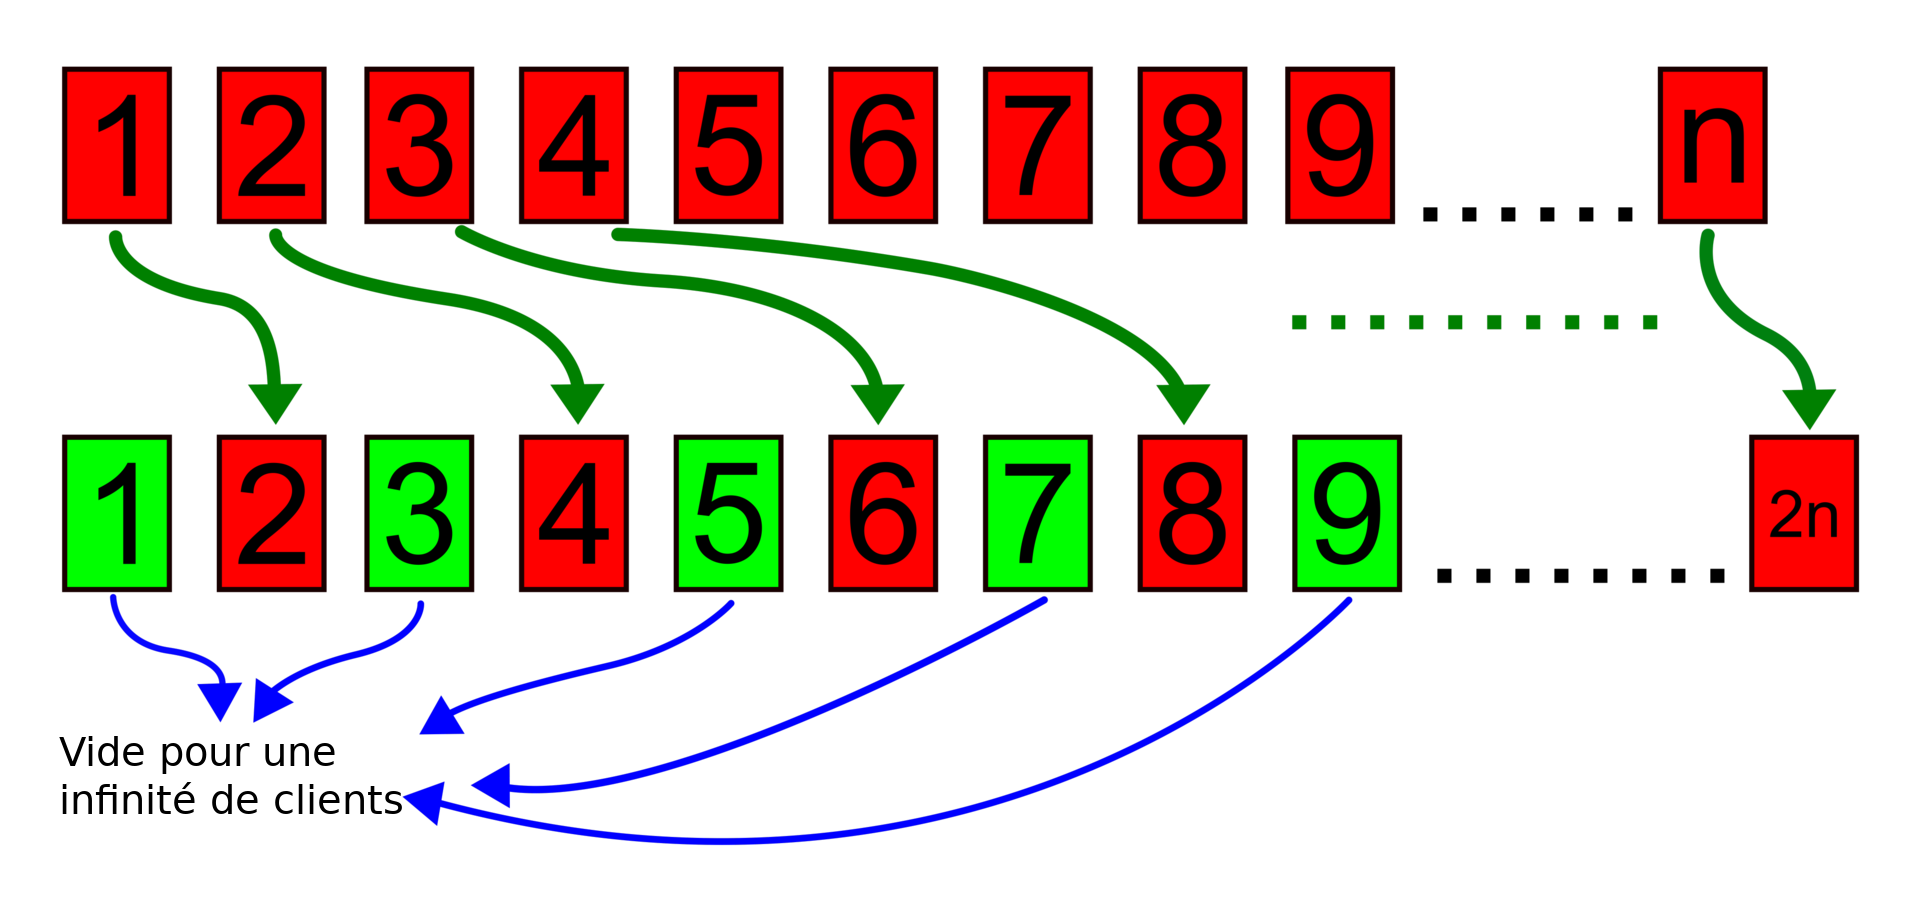
\includegraphics[width=0.7\textwidth,keepaspectratio]{hotel de hilbert.png}
    \caption{Hôtel de \bsc{Hilbert}}
    \label{fig:hotel_hilbert}
\end{figure}
\clearpage
\section{Définition générale de la dénombrabilité}
Commençons par une définition précise de ce que l'on vient de constater :
\begin{defb}{Ensemble démombrable, au plus dénombrable}{denomb}

	 Soit $E$ un ensemble infini.

	 On dit que $E$ est dénombrable ssi il existe une application $\phi~: \NN \to E $ bijective.

	 Un ensemble fini ou dénombrable est dit au plus dénombrable. \newline
	 On note par la suite $\aleph_0$, lire \emph{alèf zéro}\footnotemark, le cardinal de $\NN$.
\end{defb}
\footnotetext{Aleph, première lettre  de l'alphabet hébreu}


\section{\texorpdfstring{Dénombrabilité de 2$\NN$}{Dénombrabilité de 2N}}
\label{sec:denombrabilite_usuelle}
Il semble que l'ensemble des nombre premiers n'est pas le seul à défier notre intuition :  voici un résultat sur la dénombrabilité de  $2\NN$, l'ensemble des entiers naturels pairs.

\begin{theoremb}{Dénombrabilité de 2$\NN$}{}
	L'ensemble 2$\NN$ des entiers naturels pairs est dénombrable.
\end{theoremb}

\begin{proof}
	On construit l'application :
  \[ \deffunct{\phi}{\NN}{2\NN}{n}{2n}\]

  Cette application $\phi $ est bijective car sa réciproque est donnée par :
\[\deffunct{\phi^{-1}}{2\NN}{\NN}{k}{\frac{k}{2}}\]
	2$\NN$ est en bijection avec $\NN$, donc dénombrable de cardinal $\aleph_0$.
\end{proof}

On peut introduire un résultat plus général qui couvre toute partie de $\NN$.

\begin{theoremb}{Dénombrabilité des parties infinies de $\NN$}{}
	Toute partie $E \subseteq \NN$ infinie a le même cardinal que $\NN$.
\end{theoremb}

\begin{proof}
	On construit, par récurrence, une bijection $\phi~: \NN \to E$ telle que:

	\[\left\lbrace \begin{array}{c}
	\phi(0) = \min \{x \in E\} \\
	\forall n \in \NN, \phi(n+1) = \min \{x \in E, x > \phi(n) \}
	\end{array} \right.\]

	C'est bien une bijection~: elle est injective et surjective car $\forall k \in \NN, k \leq \phi(k)$.
\end{proof}
On en déduit le résultat suivant :
\begin{theoremb}{}{parties}
	Soient $E$ et $F$ deux ensembles.
	Si $E \subseteq F$ et si $F$ est dénombrable, alors $E$ est au plus dénombrable.
\end{theoremb}
\section{\texorpdfstring{Dénombrabilité de $\NN^2$}{Dénombrabilité de N²}}
Pour un ensemble $E$ fini de cardinal $n$, à moins que $\Card(E) = 1$, $\Card(E^2) \neq \Card(E)$. On pourrait penser que $\NN^2 $ contient plus d'élements que $\NN$.

\begin{theoremb}{Dénombrabilité de $\NN^2$}{n2_denombrable}
	$\NN^2$ est dénombrable.
\end{theoremb}

\begin{proof}
	On peut compter les couples $(n,m) \in \NN^2$ comme suit~: \par On représente ces couples sur un quart de plan cartésien.
	On part du couple $(0, 0)$. Dans la ligne suivante, on range $(1,0) $ et $(0,1)$. On continue avec $(2,0), (1,1), (0,2)$ (on parcourt la diagonale du point de coordonnées $(n,0)$ pour arriver au point de coordonnées $(0,n)$). Ce procédé est illustré dans la  \cref{fig:n_croix_n}.
	\begin{figure}[htb]
		\centering
		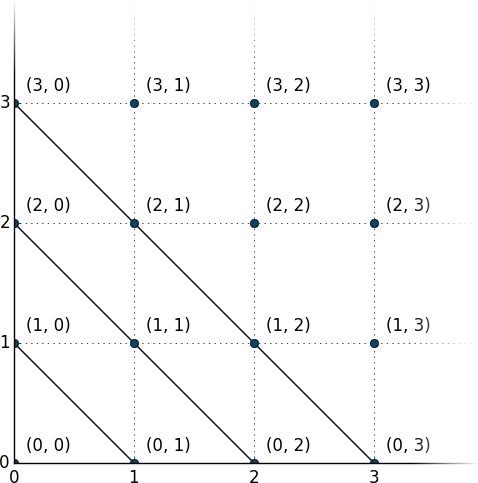
\includegraphics[scale=0.3]{n_croix_n.png}
		\caption{Dénombrabilité de $\NN^2$}
		\label{fig:n_croix_n}
	\end{figure}

	On obtient la séquence suivante~:

	\[\begin{array}{l}
		(0,0) \\
		(1,0), (0,1) \\
		(0,2), (1,1), (2,0) \\
		(3,0), (1,2), (2,1), (0,3) \\
		\cdots
	\end{array}.\]
	Plus formellement, l'application qui range les couples de cette manière est
	\[\begin{array}{cccc}
		\ & \NN \times \NN & \to & \NN \\
		\phi~: & (n,m) & \mapsto & {\underbrace{\frac{(n+m)(n+m+1)}{2}}_{\text{la place du couple dans la ligne}}} +  {\underbrace{\vphantom{\frac{(n+m)(n+m+1)}{2}} m}_{\text{la place du couple dans la colonne}}}
	\end{array}.\]


	$\phi$ est bien bijective. $\NN^2$ est bien dénombrable.
\end{proof}


Par récurrence sur $k \in \NN$, on peut montrer le théorème suivant :
\begin{theoremb}{}{nk_denombrable}
    $\NN^k$ est dénombrable.
\end{theoremb}

\begin{proof}

  Pour $k = 3$, on peut, en utilisant les notations du \cref{thm:n2_denombrable}, établir une bijection entre $\NN^2$ et $\NN^3$. Posons $h_3 : \NN^2 \to \NN^3$ telle que $h_3(n,m) = (n,\phi^{-1}(m))$. $h_3$ est bien une bijection. Soit $k \in \NN$ fixé. Supposons l'hypothèse vraie au rang $k$, i. e. $\NN^k$ est dénombrable.

  On construit une bijection entre $\NN^2$ et $\NN^{k+1}$ en posant $h_{k+1}(n_1, \dots, n_{k+1}) = (h_k(n_1, \dots, n_k),n_{k+1})$ où $h_k(n_1, \dots, n_k) \in \NN$. D'après l'hypothèse de récurrence, $\NN^k$ est dénombrable.

  On a ainsi établi une bijection entre $\NN^{k+1}$ et $\NN^2$. Or $\NN^2$ est dénombrable. Donc $\NN^k$ est dénombrable. Par récurrence, $\forall k \in \NN, \NN^k$ est dénombrable et $h_k$ est une bijection $\NN^k \to \NN$.

\end{proof}
De la dénombrabilité de $\NN^2$, on peut démontrer le théorème suivant :
\begin{theoremb}{Produit cartésien d'ensembles dénombrables}{cartesien}
	Soient $A, B, A_1, \dots, A_i, \dots, A_n$ des ensembles dénombrables.
	\begin{enumerate}
		\item Le produit cartésien $A \times B$ est dénombrable.
		\item Plus généralement, tout produit \textbf{fini} $\prod_{i=1}^{n} A_i $ est dénombrable.
	\end{enumerate}
\end{theoremb}
\begin{proof}
	Si $A$ et $B$ sont dénombrables, il existe $\phi~: A \to \NN$ et $\psi~: B \to \NN$ bijectives. On peut alors définir :
  \[ \deffunct{f}{A \times B}{\NN^{2}}{(x,y)}{(\phi(x,y),\psi(x,y))} \]

\end{proof}

$f $ est bien bijective. Donc $A \times B$ est bien dénombrable. On procède par récurrence immédiate pour $k$ ensembles.

Soit $\prod_{i =1}^k A_i$ le produit cartésien de $k$ ensembles dénombrables. Si $\forall i \in \{1,\dots,k\}, \phi_i : A_i \to \NN$ est une bijection, alors on peut construire l'application :\[ \deffunct{f} {\prod_{i=1}^k A_i}{\NN^k}{(x_1,\dots,x_k)}{(\phi_1(x_1),\dots, \phi_k(x_k))}\]
C'est une bijection de $\prod_{i=1}^k A_i $ vers $\NN^k$ qui est dénombrable. Donc $\prod_{i=1}^kA_i$ est dénombrable.


On peut encore montrer le résultat suivant :
\begin{theoremb}{Union dénombrable d'ensembles dénombrables}{union}
    Soit $(A_i)_{i \in I}$ une famille dénombrable d'ensembles dénombrables.
	Alors $A= \bigcup_{i \in I} A_i$ est dénombrable.
\end{theoremb}
\begin{proof}
	En effet, on peut écrire $\forall i \in I, A_i = \{x_{n,i}, n \in \NN\}$. Chaque élement $x_{n, i}$ est indéxé par sa position $n$ dans $A_i$ et la position $i$ de $(A_i)$ dans $I$.

	Ainsi $A = \bigcup_{i \in I} A_i = \{x_{n, i}, (n,i) \in \NN \times I\}$. Les élements $x_{n,i}$ sont indéxés par $\NN \times I$ qui est un produit cartésien d'ensembles dénombrables ($I$ est une famille indéxée par $\NN$, elle est bien dénombrable). Donc $A$ est dénombrable.
\end{proof}
\section{\texorpdfstring{Dénombrabilité de $\ZZ$ et de $\QQ$}{Dénombrabilité de Z et Q}}

Intuitivement on pourrait penser que l'ensemble des entiers $\ZZ$ a un cardinal supérieur à $\NN$ étant donné qu'il contient \enquote{deux fois plus} d'élements~: les entiers naturels et les entiers négatifs.

\begin{theoremb}{Dénombrabilité de $\ZZ$}{denz}
	L'ensemble $\ZZ$ des entiers est dénombrable.
\end{theoremb}

\begin{proof}
L'idée de la démonstration revient à écrire l'ensemble des entiers, dans l'ordre suivant~:  $\ZZ=\left\lbrace 0,1,(-1),2,(-2),3,(-3),\dots\right\rbrace$

Pour montrer que le cardinal de $\ZZ$ est bien $\aleph_0$, on définit donc l'application $\phi~: \NN \to \ZZ$ telle que
\[ \forall k \in \NN, \phi\,\colon
	\begin{dcases}
	\phi(2k)=& -k \\
	\phi(2k + 1)=& k+1
	\end{dcases}\]
	C'est bien une bijection. Donc $\ZZ$ est dénombrable.
\end{proof}
\begin{theoremb}{Dénombrabilité de $\QQ$}{denq}
	$\QQ$ est dénombrable.
\end{theoremb}
\begin{proof}
	Tout $x \in \QQ$ a un unique représentant irréductible $\frac{p}{q}$ où $p \wedge q = 1$.

	Pour établir une bijection entre $\QQ$ et $\NN$, on commence par écrire un tableau où on range $\frac{p}{q}$ à la colonne $q$ et à la ligne $p$.

	On parcourt le tableau comme c'est indiqué par les flèches dans la \cref{fig:denombQ}.

	\noindent On part de $\frac{1}{1}$ dans le tableau. On se déplace à la colonne suivante pour atteindre $\frac{1}{2}$. On parcourt le tableau diagonalement vers le bas pour atteindre $\frac{2}{1}$, on descend d'une case pour obtenir $\frac{3}{1}$ et on parcourt le tableau en diagonale vers le haut jusqu'à atteindre $\frac{1}{3}$, etc.

	On s'aperçoit que chaque nombre rationnel dans le tableau a un et un seul rang $r$ (sa place dans le tableau). L'application $\phi$ qui range les rationnels $x \in \QQ$ dans le tableau \cref{fig:denombQ} est donc une bijection.
\end{proof}
\begin{figure}[!htb]
    \centering
\begin{tikzpicture}
\tikzstyle{keepstyle} =[rectangle, rounded corners, draw, fill=white]
\node at (0,0) {$\vdots$};
\node[keepstyle] (51) at (0,1) {$\frac{5}{1}$};
\node[keepstyle] (41) at (0,2) {$\frac{4}{1}$};
\node[keepstyle] (31) at (0,3) {$\frac{3}{1}$};
\node[keepstyle] (21) at (0,4) {$\frac{2}{1}$};
\node[keepstyle] (11) at (0,5) {$\frac{1}{1}$};
\node at (1,0) {$\vdots$};
\node[keepstyle] (52) at (1,1) {$\frac{5}{2}$};
\node at (1,2) {$\frac{4}{2}$};
\node[keepstyle] (32) at (1,3) {$\frac{3}{2}$};
\node at (1,4) {$\frac{2}{2}$};
\node[keepstyle] (12) at (1,5) {$\frac{1}{2}$};
\node at (2,0) {$\vdots$};
\node at (2,1) {$\frac{5}{3}$};
\node[keepstyle] (43) at (2,2) {$\frac{4}{3}$};
\node at (2,3) {$\frac{3}{3}$};
\node[keepstyle] (23) at (2,4) {$\frac{2}{3}$};
\node[keepstyle] (13) at (2,5) {$\frac{1}{3}$};
\node at (3,0) {$\vdots$};
\node at (3,1) {$\frac{5}{4}$};
\node at (3,2) {$\frac{4}{4}$};
\node[keepstyle] (34) at (3,3) {$\frac{3}{4}$};
\node at (3,4) {$\frac{2}{4}$};
\node[keepstyle] (14) at (3,5) {$\frac{1}{4}$};
\node at (4,0) {$\vdots$};
\node  at (4,1) {$\frac{5}{5}$};
\node at (4,2) {$\frac{4}{5}$};
\node at (4,3) {$\frac{3}{5}$};
\node[keepstyle] (25) at (4,4) {$\frac{2}{5}$};
\node[keepstyle] (15) at (4,5) {$\frac{1}{5}$};
\node at (5,0) {$\vdots$};
\node  at (5,1) {$\frac{5}{6}$};
\node at (5,2) {$\frac{4}{6}$};
\node at (5,3) {$\frac{3}{6}$};
\node at (5,4) {$\frac{2}{6}$};
\node[keepstyle] (16) at (5,5) {$\frac{1}{6}$};
\node at (6,1) {$\cdots$};
\node at (6,2) {$\cdots$};
\node at (6,3) {$\cdots$};
\node at (6,4) {$\cdots$};
\node at (6,5) {$\cdots$};
\draw [-latex,red, thick] (11) -- (12);
\draw [-latex, red, thick] (12) -- (21);
\draw [-latex, red, thick] (21) -- (31);
\draw [-latex, red, thick] (31) -- (13);
\draw [-latex, red, thick] (13) -- (14);
\draw [-latex, red, thick] (14) -- (23);
\draw [-latex, red, thick] (23) -- (32);
\draw [-latex, red, thick] (32) -- (41);
\draw [-latex, red, thick] (41) -- (51);
\draw [-latex, red, thick] (51) -- (15);
\draw [-latex, red, thick] (15) -- (16);
\draw [-latex, red, thick] (16) -- (25);
\draw [-latex, red, thick] (25) -- (34);
\draw [-latex, red, thick] (34) -- (43);
\draw [-latex, red, thick] (43) -- (52);
\end{tikzpicture}
\caption{Dénombrabilité de $\QQ$}
    \label{fig:denombQ}
  \end{figure}
\clearpage
  \section*{Complément : dénombrabilité de l'ensemble des polynômes à coefficients entiers}
  \addcontentsline{toc}{chapter}{Complément : dénombrabilité de l'ensemble des polynômes à coefficients entiers}% fait un chapitre sans numéro en table des matières
On se propose d'appliquer toutes les notions que nous venons de voir pour démontrer l'assertion suivante : l'ensemble des polynômes à coefficients entiers est dénombrable. Ce résultat peut paraître surprenant. En effet, étant donné qu'un polynôme est caractérisé par ses coefficients, on pense, intuitivement, que l'on peut trouver plus de \enquote{combinaisons d'entiers} pour caractériser un polynôme que d'entiers.

Soit $P \eqdef \sum_{k = 1}^d a_k X^k $, où $d = \operatorname{deg}(P)$. Notons $\ZZ_d[X] = \{P \in \ZZ[X], \operatorname{deg}(P) \leq d \}.$
On pose  $(a_0, \dots, a_d) $ une suite de ses coefficients. On définit une application
\[\deffunct{\phi}{\ZZ[X]}{\ZZ^{d+1}}{P}{(a_{0},\dots,a_{d}  )}\]
$\phi$ est une injection, car $\forall Q \in \ZZ[X]$, où $Q \displaystyle\eqdef \sum_{k=1}^d b_k X^k,$ \[{{P = Q} \iff {\forall k \in \left\lBrack 1;d\right\rBrack, a_k = b_k}}.\]C'est une surjection : à toute suite de coefficients $(a_0,\dots, a_d)$ on peut associer un polynôme ${P = \sum_{k=1}^d a_k X^k}$. Or on a vu que comme $\ZZ$ est dénombrable, $\ZZ^{d+1}$ l'est aussi par extension,%\sidepar{car $\NN^{d+1}$ est dénombrable}%
donc $\ZZ_d[X]$ est dénombrable Mais $\ZZ[X] = \bigcup_{d \in \NN} \ZZ_d[X]$. On a vu que toute réunion dénombrable d'ensembles dénombrables est dénombrable. Donc $\ZZ[X]$ est dénombrable.

\section*{\texorpdfstring{Application : bijection entre deux sous-ensembles de $\QQ$}{}}

Nous allons appliquer les concepts vu récemment pour répondre à la question suivante :

\[X = \QQ \cap [0,1] \text{ est-il plus grand que } Y = \QQ \cap \left]0,1\right[ \text{ ?}\]

Naturellement, on peut penser que, comme 0 et 1 sont des rationnels, ils sont dans $X$ et qu'$X$ contient deux éléments de plus que $Y$.

Montrons que $ X = \QQ \cap [0,1]$ et $ Y = \QQ \cap \left]0,1\right[$ sont en bijection.
\begin{proof}
$X $ et $Y$ sont des sous-ensembles de $\QQ$. Donc ils sont dénombrables. Ainsi \[\exists \phi : \NN \to X \text{ et } \psi : \NN \to Y\text{, bijectives.}\]

Ainsi on peut construire une bijection $\gamma \eqdef \phi^{-1} \circ \psi :\, X \to Y$, donc $X$ et $Y$ sont équipotents.
\end{proof}
Ce problème est une illustration du paradoxe de \bsc{Hilbert} : si $A$ et $B$ sont~dénombrables, peu importe le nombre \emph{fini} d'élements que l'on ajoute à $A$ ou à $B$, ils auront  la même puissance~$\aleph_0$.
\chapter*{Conclusion}

Nous l'avons vu, les propriétés de l'infini dénombrable défient l'intuition. Même les plus grands mathématiciens furent étonnés lorsqu'ils découvrirent ces résultats. \bsc{Cantor} écrivit dans sa correspondance à \bsc{Dedekind} à ce propos : \epigraph{\textit{Je le vois, mais je ne le crois pas\textellipsis}\newline [en français dans le texte en allemand]}{\bsc{Georg Cantor}\\29 juin 1877~\cite{Volken2003}.} Pourtant ces propriétés bizarres et contre-intuitives à premier abord sont révélatrices de la complexité et de la beauté des mathématiques.

L'étude de la dénombrabilité a été notre première (modeste) contribution à la Science. Il nous a permis d'appliquer les connaissances agrégées durant notre cursus universitaire et de développer notre autonomie et notre curiosité.

Comme ce sera indiqué dans la prochaine présentation, l'ensemble des réels n'est pas dénombrable. L'argument de la diagonale de Cantor qui construit la démonstration de cette propriété peut être appliqué dans le domaine de l'informatique, notamment pour montrer l'indécidabilité du problème de l'arrêt.

\addcontentsline{toc}{chapter}{Conclusion}
\appendix
\appendixpage
\backmatter
\chapter{Manuel des commandes}
Annexe à lire avec \texttt{main.tex} et \texttt{personalisation.tex} sous les yeux.
\begin{theoremb}{Exemple}{exem}
\(\alpha\beta\gamma ABCD=\)
\end{theoremb}
\begin{remarkb}{Remarque}{rema}
\(a\)
\end{remarkb}
\begin{noteb}{Note}{not}
$a$
\end{noteb}
\begin{defb}{Définition}{def}
$a$
\end{defb}
\vspace{-\parskip}
\begin{proof}
\proofpart{test}
\[TRUC\]
\proofpart{}
\[MACHIN\]
\proofpart*{test}
\[BIDULE\]
\end{proof}
\Cref{thm:exem}, \cref{rem:rema}, \cref{note:not} \cref{def:def}
$\restriction{f}{A}$ $\corestriction{f}{A}$ $\transp{\left(\transp{M^{2}}\right)}$

\noindent Définition de fonctions : \verb|\displaystyle ($$ $$ / \[ \])| vs \verb|\textstyle ($ $)| :
\[\deffunct{f}{E}{F}{x}{f(x)} \text{ vs. }\textstyle  \deffunct{f}{E}{F}{x}{f(x)}\]--
%\listoffigures
%\printindex
\nocite{*}
%\raggedright
\printbibliography
\end{document}
%%% Local Variables:
%%% mode: latex
%%% TeX-engine: luatex
%%% TeX-master: t
%%% End:
